\documentclass[11pt,a4paper]{article}
\usepackage{fontspec}
\setmainfont{TeX Gyre Pagella}
\newfontfamily\headfont{Inter}[UprightFont=*-ExtraBold,BoldFont=*-ExtraBold,Extension=.otf,Path=/usr/share/fonts/opentype/inter/]
\usepackage[a4paper,margin=2.3cm]{geometry}
\usepackage{graphicx,booktabs,float,caption,array,xcolor}
\usepackage[hidelinks]{hyperref}
\usepackage{titlesec}
\usepackage[round]{natbib}
\usepackage{setspace}
\setstretch{1.05}
\renewcommand{\topfraction}{0.9}
\renewcommand{\bottomfraction}{0.8}
\renewcommand{\textfraction}{0.1}
\renewcommand{\floatpagefraction}{0.75}
\setlength{\parindent}{0pt}
\setlength{\parskip}{0.55em}
\titleformat{\section}{\headfont\Large}{\thesection}{0.8em}{}
\titleformat{\subsection}{\headfont\large}{\thesubsection}{0.8em}{}
\captionsetup{font=small,labelfont=bf}
\urlstyle{same}
\hypersetup{pdftitle={Where the Animals Are: the World's Farm Animals, Mapped},pdfauthor={Tristan Hotham}}

\begin{document}
\begin{center}
{\Large\bfseries Where the Animals Are\par}
\vspace{0.4em}
{\large The world's cattle, sheep, goats, pigs, chickens and other farm animals,\\mapped every 10 km and counted by country, 1961 to 2024\par}
\vspace{1.2em}
{\large Tristan Hotham\par}
\vspace{0.3em}
{\small Independent researcher\\
ORCID: 0000-0003-4931-9349\\
DOI: \href{https://doi.org/10.5281/zenodo.23842985}{https://doi.org/10.5281/zenodo.23842985}\par}
\vspace{0.8em}
2026
\end{center}

\begin{quote}
\small
\begin{center}\textbf{Abstract}\end{center}
Most of the large animals alive on Earth are farm animals, but their geography is rarely shown in one place. I combine the FAO's Gridded Livestock of the World (GLW 4), which estimates the number of cattle, buffaloes, sheep, goats, pigs, chickens, ducks and horses in every 5 arc minute cell in 2015, with FAOSTAT's national livestock counts for 1961 to 2024 and World Bank population figures, and publish the result as an open interactive atlas. In 2024 there were about 35.3 billion farm animals alive at once, 4.3 for every person: 3.6 birds and 0.67 mammals per person. Since 1961 chickens have multiplied 7.1 times and goats 3.4 times, against 2.7 times for people, while cattle per person fell from 0.31 to 0.19. Farm mammals outnumber people in 40 of 159 countries of a million people or more, most of all in Mongolia (16.4 per person). Some animals belong largely to one country: China has 44\% of the world's pigs and India 53\% of its buffaloes. On the grid, half of all pigs live on 1.3\% of the world's land and half of all cattle on 5.9\%. Weighted by livestock units, cattle are the main farm animal in 127 of 194 countries and on 42\% of the world's land. A closer look at Britain and Ireland separates the sheep hills of Wales and the Borders from the dairy pastures of the west and the pig and poultry plains of the east.

\textbf{Keywords:} livestock; cattle; sheep; goats; pigs; poultry; FAOSTAT; Gridded Livestock of the World; mapping; open data
\end{quote}

\section{Introduction}
Farm animals are among the most numerous large animals on Earth, and the land they need is vast: permanent meadows and pastures make up 66\% of the world's agricultural land in FAOSTAT's land use statistics. Yet the everyday picture of where farm animals live is patchy: sheep in New Zealand, cattle in Argentina, pigs in Denmark. This study puts the world's main farm animals on one map and asks four simple questions. How many are there, and how has that changed since 1961? Where do animals outnumber people? How concentrated are they, between countries and on the ground? And which animal dominates each place?

The sources are well known in agricultural research but less so outside it. The Food and Agriculture Organization's FAOSTAT database \citep{faostat} reports the number of animals alive in each country every year. The Gridded Livestock of the World \citep{gilbert2018,nicolas2016,robinson2014} turns sub-national census counts into a global grid of densities with a statistical model. Neither is new. The contribution here is descriptive and practical: a consistent set of country and grid statistics, an interactive atlas at \url{https://maps.tristanhotham.com/livestock-map/} where anyone can switch between animals and zoom to their own area, and open derived data and code.

\section{Data}
\textbf{Gridded Livestock of the World (GLW 4).} Global rasters at 5 arc minutes (about 10 km at the equator) for cattle, buffaloes, sheep, goats, pigs, chickens, ducks and horses for the reference year 2015, distributed by FAO on the Harvard Dataverse under CC BY 4.0 \citep{glw4}. I use the dasymetric (`Da') layers, in which each sub-national census total is shared among the cells inside its census area in proportion to densities predicted by random forest models from climate, vegetation, land cover, terrain, travel time to cities and human population \citep{nicolas2016,gilbert2018}. The cell area raster distributed with GLW gives densities per km\textsuperscript{2}. Summed over the world, the grid matches FAOSTAT's 2015 totals closely (100.3\% for cattle, 99.8\% for pigs, 105.5\% for horses).

\textbf{FAOSTAT.} Bulk downloads of the Crops and Livestock Products domain (QCL), the Livestock Patterns domain (EK) and the Land Use domain (RL), retrieved in 2026 \citep{faostat}. From QCL I keep the element `Stocks' (animals alive, in head or thousand head) for eighteen items: cattle, buffaloes, sheep, goats, pigs, chickens, ducks, geese, turkeys, other birds, horses, asses, mules and hinnies, camels, other camelids, rabbits and hares, other rodents and beehives. From EK I take stocks expressed in livestock units, and from RL each country's land area and agricultural land.

\textbf{Population and geography.} World Bank total population by country and year \citep{wbpop}, Natural Earth countries and populated places \citep{naturalearth}, and UK counties (ceremonial counties in England, preserved counties in Wales, council areas in Scotland and Northern Ireland as one unit) from ONS and partner boundaries.

\begin{table}[tbp]\centering\small\caption{World farm animals alive in 1961 and 2024 (FAOSTAT stocks, millions), growth, and animals per 100 people in 2024.}\label{tab:world}\begin{tabular}{lrrrr}\toprule Animal & 1961 & 2024 & Multiple & Per 100 people\\\midrule
Chickens & 3,906.2 & 27,680.7 & 7.09 & 340.0\\
Cattle & 942.1 & 1,578.6 & 1.68 & 19.4\\
Sheep & 993.6 & 1,362.6 & 1.37 & 16.7\\
Ducks & 193.4 & 1,274.8 & 6.59 & 15.7\\
Goats & 348.6 & 1,187.5 & 3.41 & 14.6\\
Pigs & 406.1 & 962.4 & 2.37 & 11.8\\
Geese & 36.6 & 382.5 & 10.44 & 4.7\\
Turkeys & 204.2 & 243.5 & 1.19 & 3.0\\
Buffaloes & 88.3 & 212.0 & 2.40 & 2.6\\
Rabbits and hares & 98.0 & 210.1 & 2.14 & 2.6\\
Horses & 62.2 & 56.2 & 0.90 & 0.7\\
Donkeys & 37.0 & 53.9 & 1.46 & 0.7\\
Camels & 12.9 & 44.3 & 3.44 & 0.5\\
Other rodents (guinea pigs) & 20.7 & 18.9 & 0.91 & 0.2\\
Llamas and alpacas & 5.3 & 8.6 & 1.63 & 0.1\\
Mules and hinnies & 10.5 & 7.7 & 0.74 & 0.1\\
Other birds (pigeons, quail) & n/a & 24.2 & n/a & 0.3\\
\midrule People & 3,062.8 & 8,140.9 & 2.66 & \\\bottomrule\end{tabular}\end{table}

\section{Methods}
\textbf{Matching countries.} FAOSTAT areas are matched to Natural Earth countries through UN M49 codes. FAOSTAT's aggregate regions and its `China' total (which adds Taiwan, Hong Kong and Macao to the mainland) are excluded from country tables; China means mainland China. Former states, namely the USSR, Yugoslavia, Czechoslovakia, Serbia and Montenegro, Ethiopia PDR, the former Sudan and Belgium-Luxembourg, are counted in FAOSTAT's world totals but have no present-day country here, so series for their successors begin when FAOSTAT begins reporting them. French overseas departments reported separately by FAOSTAT are not joined to France. Per person figures divide by the World Bank population of the same year. A country is listed among those where animals `outnumber people' only if it has at least a million people.

\textbf{Livestock units.} To compare a cow with a chicken I use FAOSTAT's own livestock unit factors. Dividing each country's stocks in livestock units (EK, latest year 2023) by its head count (QCL, same year) gives a country specific factor for cattle, buffaloes, sheep, goats, pigs, chickens, horses, asses, mules and camels; ducks take the chicken factor, and countries without a factor take the world average. The world averages are 0.64 for cattle, 0.53 for buffaloes, 0.10 for sheep, 0.10 for goats, 0.25 for pigs and 0.01 for chickens. The `main animal' of a country or cell is the one with most livestock units. In the grid, each cell takes the factors of its country (cells outside every country outline take those of the nearest country), and cells with fewer than one livestock unit per km\textsuperscript{2} are left without a main animal.

\textbf{Concentration.} For each animal, cells on land (Antarctica excluded) are sorted from densest to least dense, and I report the smallest share of the world's land area that holds half and nine tenths of the animals. The densest place for each animal is the cell with the highest average density over a 3 by 3 cell window.

\textbf{UK counties.} County outlines are rasterised at 1/120 degree, ten times finer than the grid, to give the fraction of each grid cell in each county. Animals in a UK cell are shared among counties by those fractions, so cells along the coast keep all their animals on land. County totals therefore add up exactly to the grid's UK total.

\textbf{Page grids.} For the interactive atlas, densities are coded on a logarithmic scale into 8 bit PNG images (one animal per colour channel) and decoded in the browser; values read from the map are within about five per cent of the grid.

\section{Results}
\subsection{How many, and how they have changed}
In 2024 FAOSTAT counts about 35.3 billion farm animals alive at once, 4.3 for each of 8.1 billion people (Table~\ref{tab:world}). Birds make up 29.6 billion of them, 93\% chickens; mammals 5.5 billion. Since 1961 people have multiplied 2.7 times, chickens 7.1 times, ducks 6.6 times, goats 3.4 times and camels 3.4 times, while cattle (1.7) and sheep (1.4) grew more slowly than people and horses (0.90) and mules (0.74) declined (Figure~\ref{fig:growth}). Asia's share of the world's chickens rose from 28\% to 61\%, and Africa and Asia now hold 95\% of all goats. The world's pig herd peaked in 2015; when African swine fever reached China, its herd fell by 28\% between 2018 and 2019 (118 million pigs) and the world herd by 12\%. By 2024 China's herd was back to 427 million.

\begin{figure}[tbp]\centering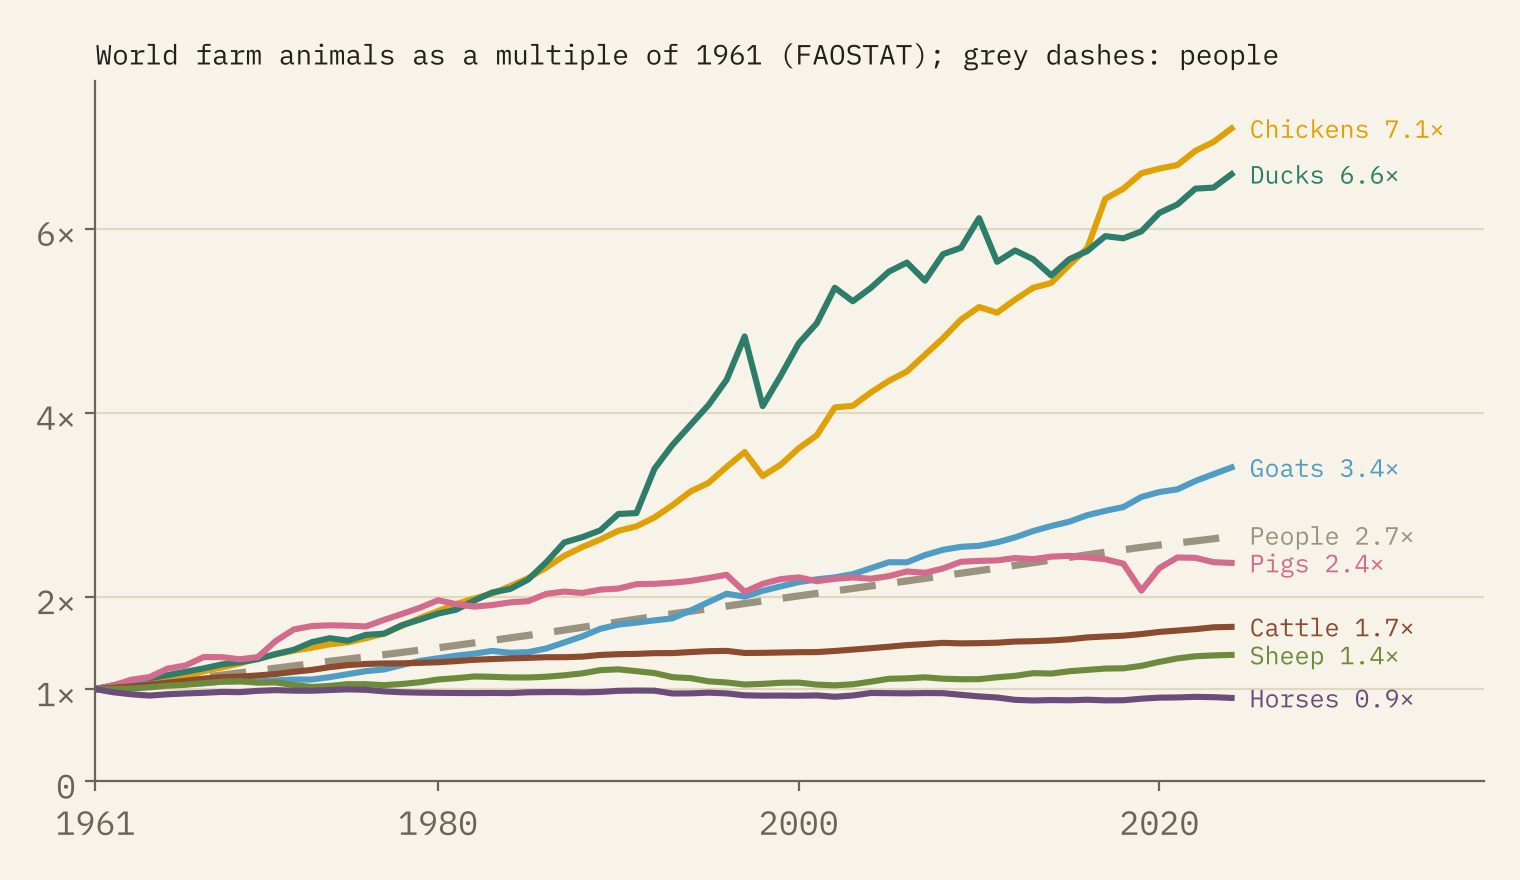
\includegraphics[width=\textwidth]{f_growth.png}
\caption{World stocks of the main farm animals as a multiple of 1961, with world population (FAOSTAT; World Bank).}\label{fig:growth}\end{figure}

\subsection{Where they live}
Figure~\ref{fig:species} maps six animals from the grid. Cattle are the most widespread, covering the grasslands and farmland of every continent; sheep and goats follow the drylands, from the Sahel and the Horn of Africa through the Middle East to Central Asia, with sheep also in Europe, southern Africa, Australia, New Zealand and Patagonia; pigs and chickens follow people and feed, densest in eastern China, Europe and the eastern United States; buffaloes are almost entirely Asian.

\begin{figure}[tbp]\centering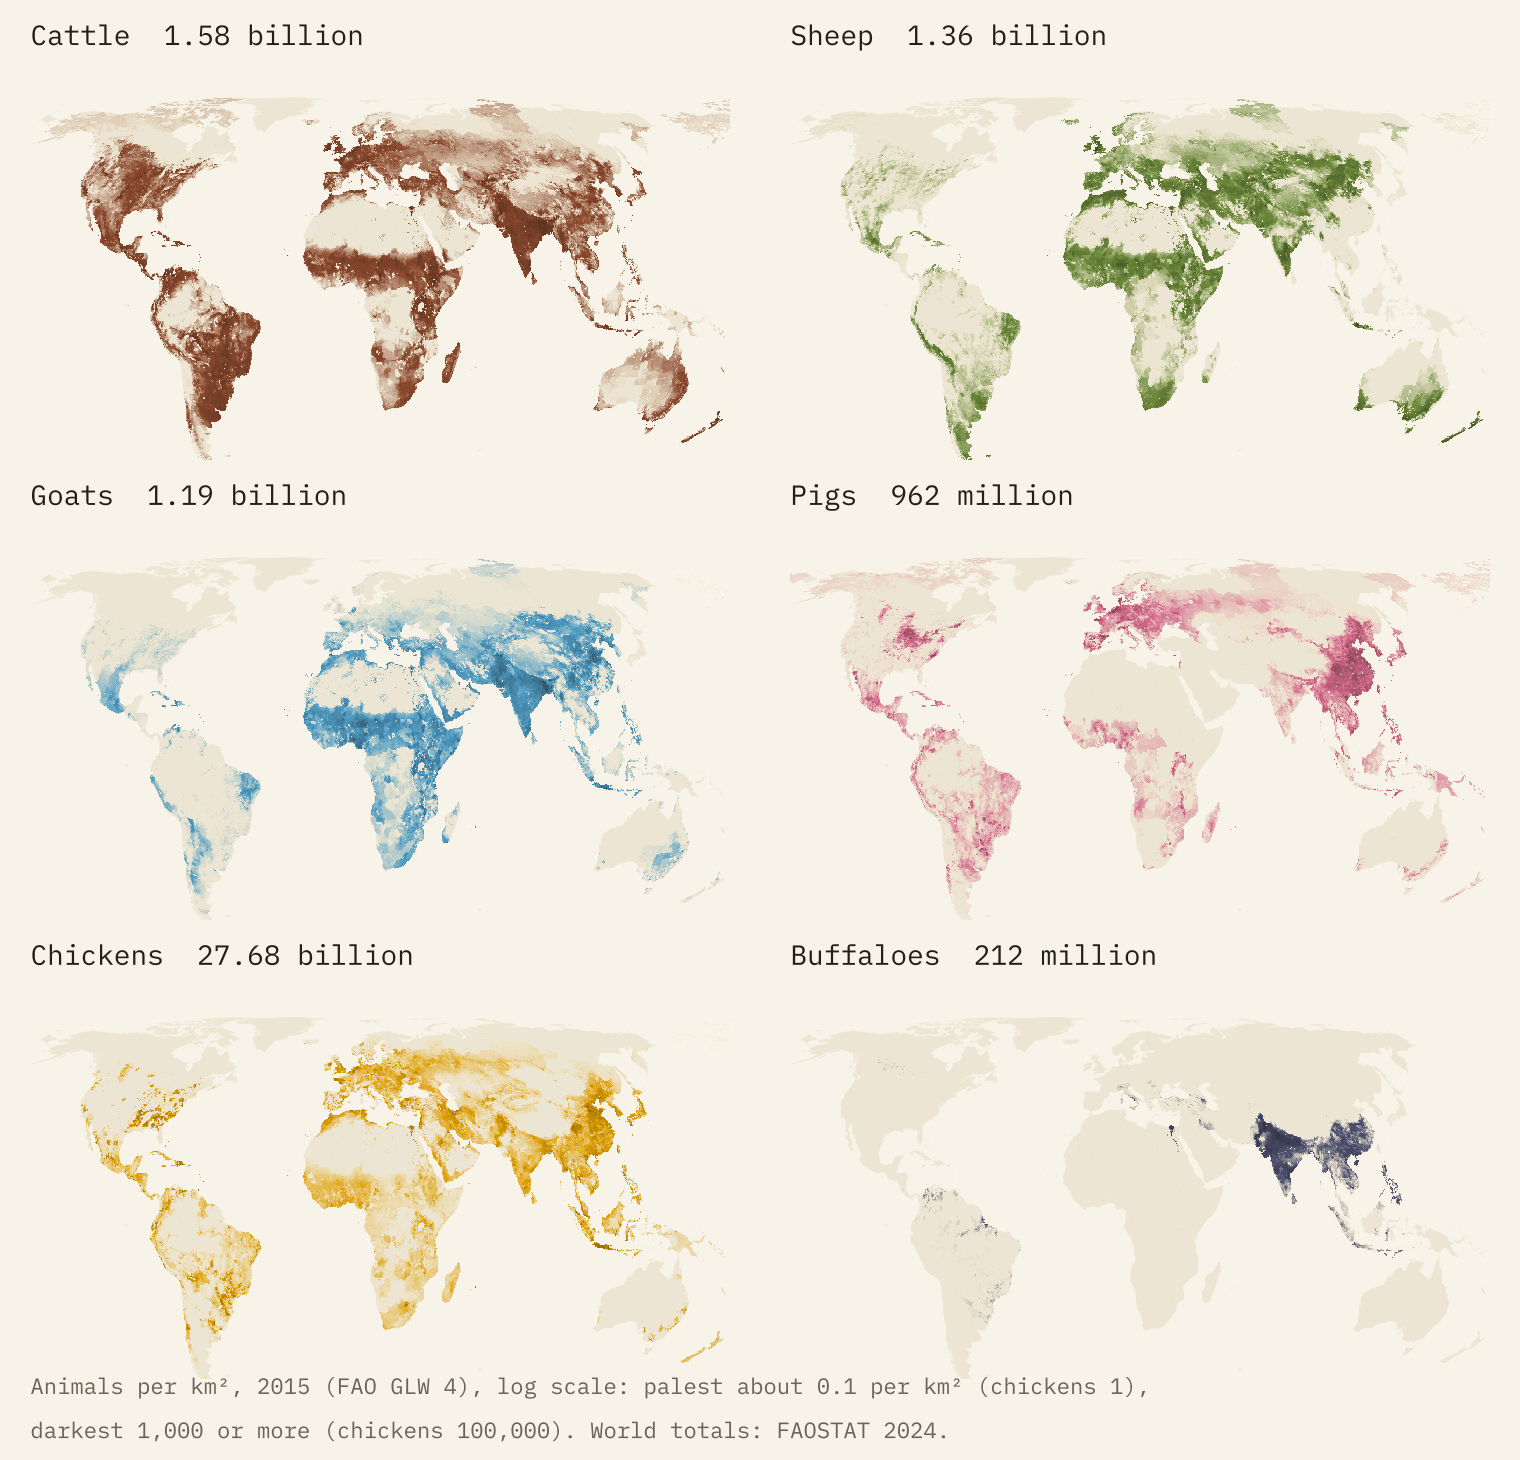
\includegraphics[width=\textwidth]{f_species.png}
\caption{Density of six farm animals in 2015 (GLW 4, dasymetric layer), animals per km\textsuperscript{2} on a log scale. Titles give FAOSTAT world totals for 2024.}\label{fig:species}\end{figure}

\subsection{Where animals outnumber people}
Farm mammals outnumber people in 40 of the 159 countries with a million people or more (Figure~\ref{fig:outnumber}, Table~\ref{tab:pp}). Mongolia has 16.4 per person, including 6.5 goats and 6.9 sheep, the most of both anywhere; its goat herd has grown 4.1 times since 1961. Chad follows with 7.4, then New Zealand (6.3), Uruguay (5.4) and Australia (4.3). Uruguay has the most cattle per person (3.5), and Denmark is the only country of a million people or more with more pigs than people (1.9). Chickens outnumber people in 110 of these countries. New Zealand's sheep flock peaked in 1982 at 70.3 million (22.3 per person) and has since fallen by 66\% to 23.6 million (4.5 per person), while its cattle herd grew by about a fifth (Figure~\ref{fig:nz}).

\begin{figure}[tbp]\centering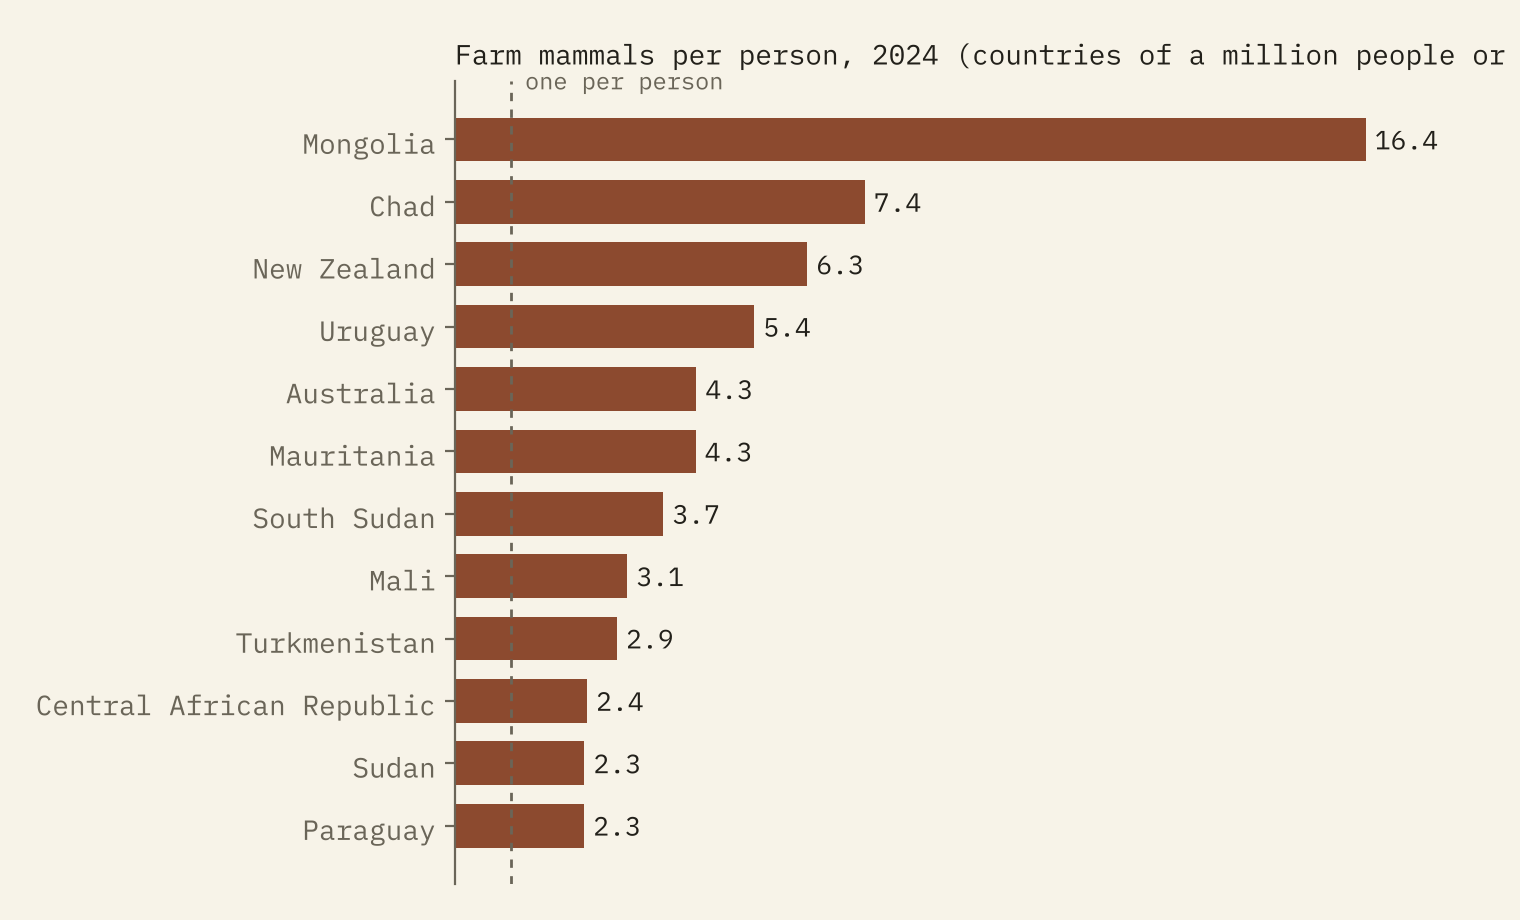
\includegraphics[width=.9\textwidth]{f_outnumber.png}
\caption{Farm mammals (cattle, buffaloes, sheep, goats, pigs, horses, asses, mules, camels, llamas and alpacas) per person, 2024, countries of a million people or more.}\label{fig:outnumber}\end{figure}

\begin{table}[tbp]\centering\small\caption{Countries with most farm mammals per person, 2024 (countries of a million people or more).}\label{tab:pp}\begin{tabular}{lrrrrrrr}\toprule Country & People (m) & Mammals & Cattle & Sheep & Goats & Camels & Horses\\\midrule
Mongolia & 3.5 & 16.4 & 1.44 & 6.95 & 6.50 & 0.14 & 1.33\\
Chad & 20.3 & 7.4 & 1.95 & 2.23 & 2.29 & 0.56 & 0.08\\
New Zealand & 5.3 & 6.3 & 1.80 & 4.46 & 0.02 & 0.00 & 0.01\\
Uruguay & 3.4 & 5.4 & 3.53 & 1.67 & 0.01 & 0.00 & 0.12\\
Australia & 27.2 & 4.3 & 1.12 & 2.92 & 0.20 & 0.00 & 0.01\\
Mauritania & 5.2 & 4.3 & 0.39 & 2.17 & 1.38 & 0.30 & 0.01\\
South Sudan & 11.9 & 3.7 & 1.20 & 1.20 & 1.31 & 0.00 & 0.00\\
Mali & 24.5 & 3.1 & 0.57 & 1.00 & 1.38 & 0.06 & 0.03\\
Turkmenistan & 7.5 & 2.9 & 0.34 & 1.90 & 0.64 & 0.02 & 0.00\\
Central African Republic & 5.3 & 2.4 & 0.91 & 0.08 & 1.16 & 0.00 & 0.00\\
Sudan & 50.4 & 2.3 & 0.62 & 0.81 & 0.63 & 0.10 & 0.02\\
Paraguay & 6.9 & 2.3 & 1.97 & 0.05 & 0.02 & 0.00 & 0.03\\
\bottomrule\end{tabular}\end{table}

\begin{figure}[tbp]\centering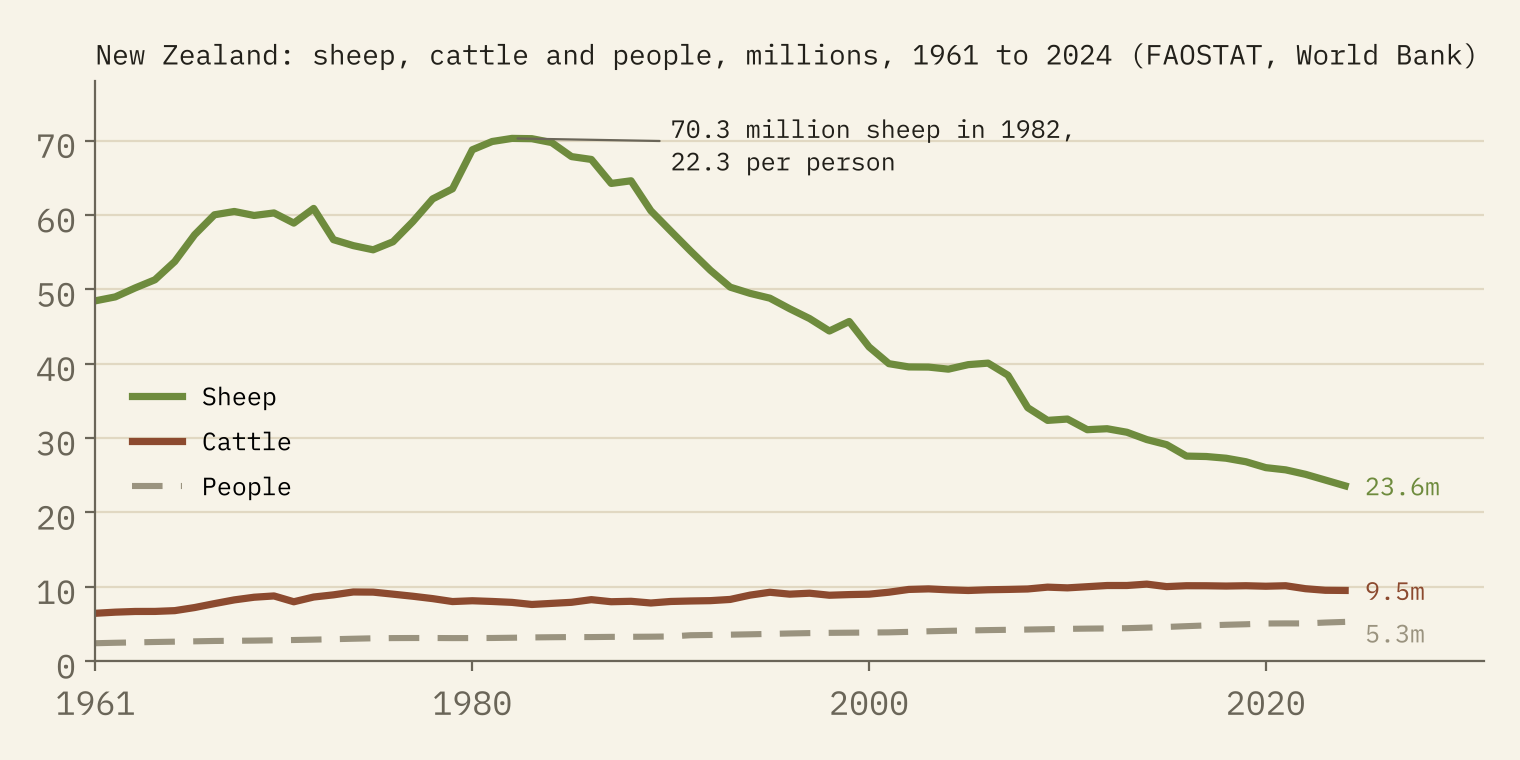
\includegraphics[width=.9\textwidth]{f_new_zealand.png}
\caption{New Zealand's sheep, cattle and people, 1961 to 2024 (FAOSTAT; World Bank).}\label{fig:nz}\end{figure}

\subsection{Concentration}
Between countries, poultry other than chickens, pigs and buffaloes are the most concentrated (Figure~\ref{fig:conc}): China has 87\% of the world's geese, 65\% of its ducks and 44\% of its pigs; India has 53\% of the buffaloes, and India, Pakistan and China together 89\%. Chad has 26\% of the world's camels. The largest herds of cattle (Brazil, 15\%), sheep (China, 13\%) and horses (Mexico, 11\%) hold much smaller shares.

On the ground the contrast is between grazing animals and housed ones (Figure~\ref{fig:land}). Half of the world's pigs live on 1.3\% of its land, half of its chickens on 1.4\% and half of its buffaloes on 0.5\%, against 3.8\% for sheep and 5.9\% for cattle. The densest pig cells are in the south-east of the Netherlands, around Eindhoven (about 3,449 pigs per km\textsuperscript{2}).

\begin{figure}[tbp]\centering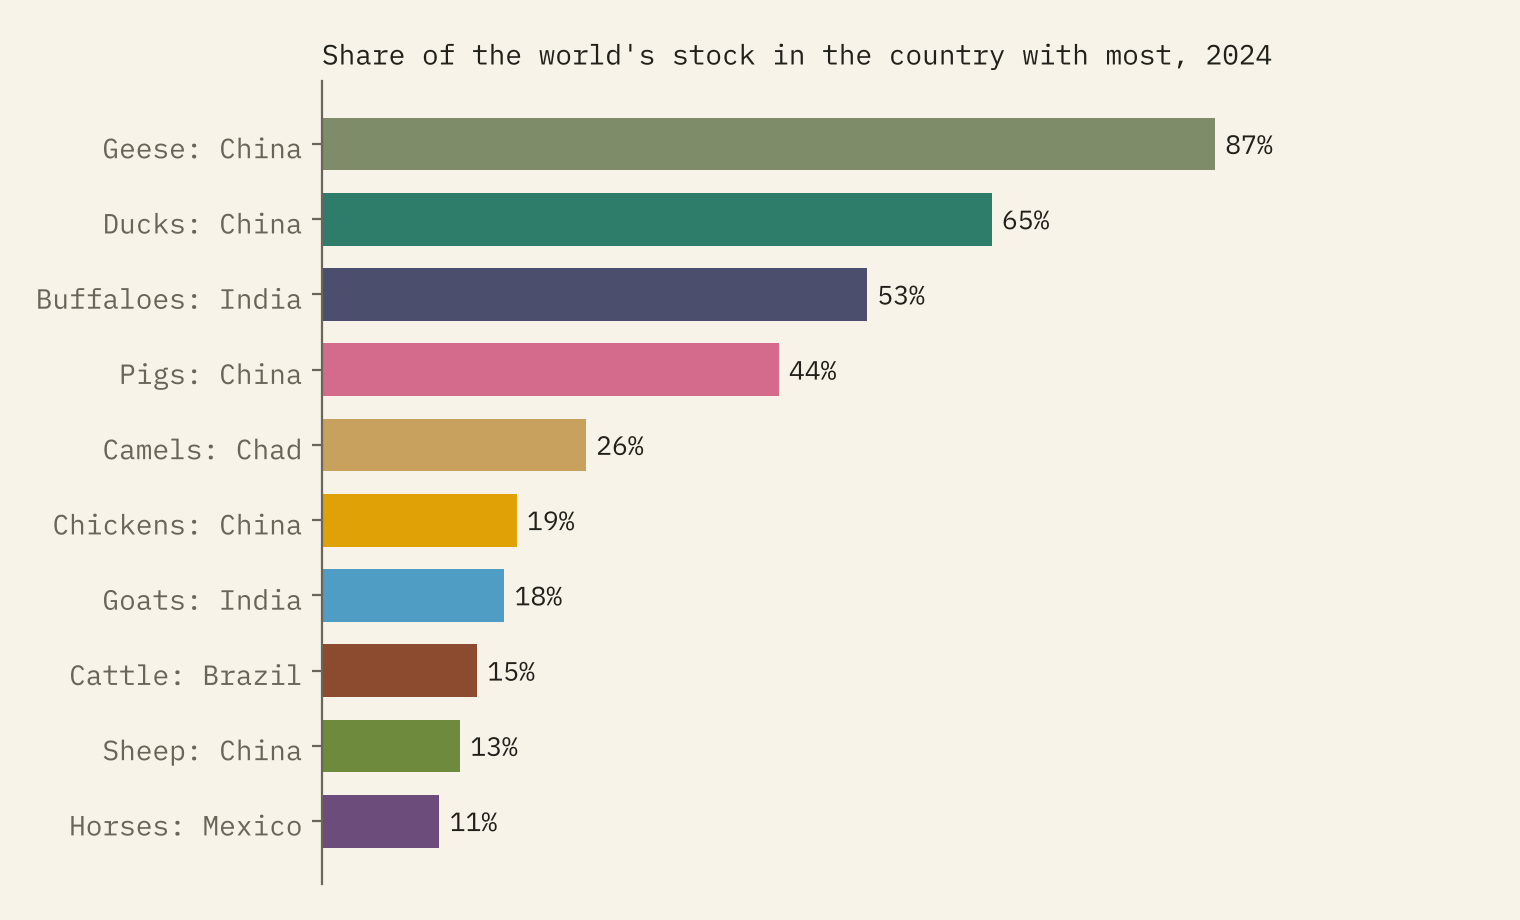
\includegraphics[width=.9\textwidth]{f_concentration.png}
\caption{Share of the world's stock held by the country with the most, 2024 (FAOSTAT).}\label{fig:conc}\end{figure}

\begin{figure}[tbp]\centering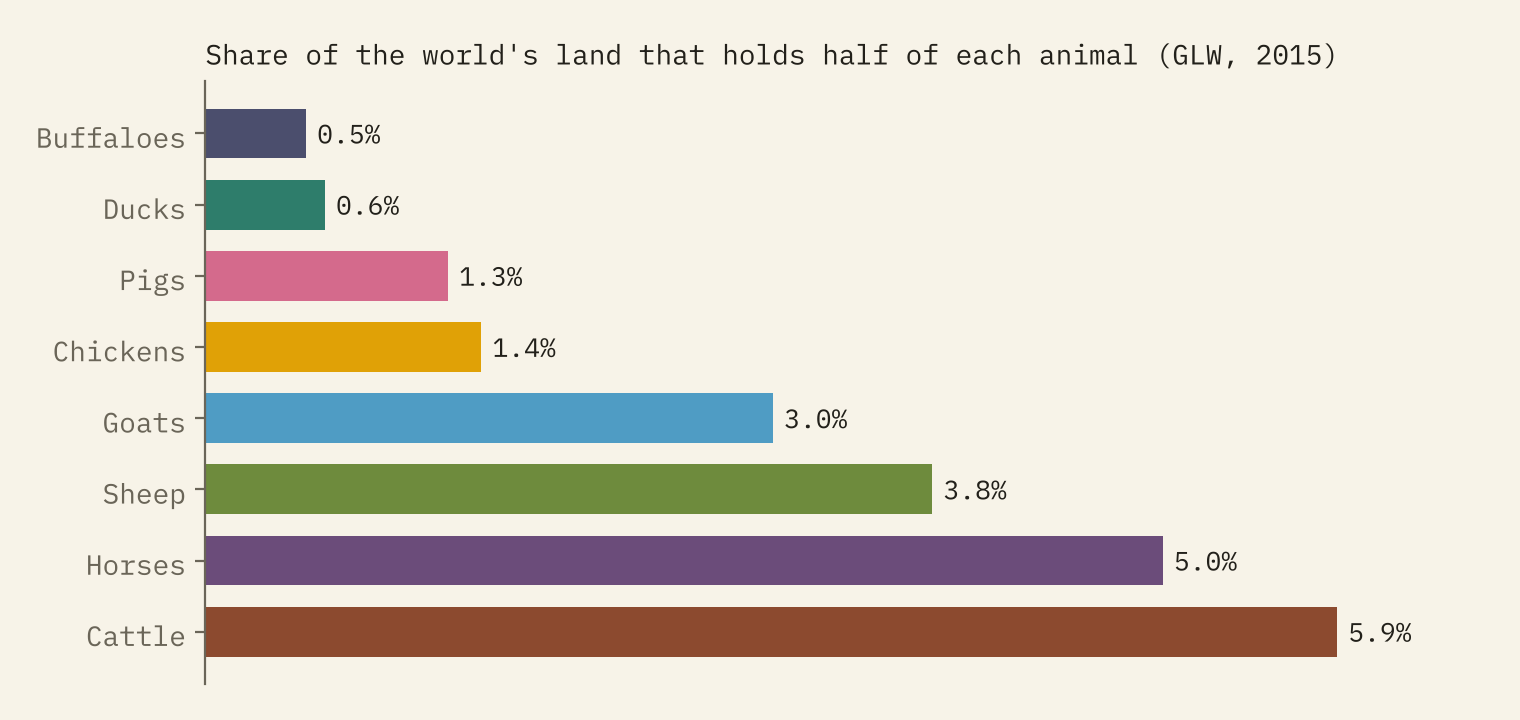
\includegraphics[width=.9\textwidth]{f_land_half.png}
\caption{The smallest share of the world's land (Antarctica excluded) that holds half of each animal, counting the densest cells first (GLW 4, 2015).}\label{fig:land}\end{figure}

\subsection{The main animal}
Weighted by livestock units, cattle are the main farm animal in 127 of 194 countries, chickens in 33, pigs in 22, sheep in 8, and goats and camels in 2 each; across all countries cattle make up 51\% of livestock units, chickens 14\% and pigs 12\%. On the grid (Figure~\ref{fig:main}) cattle lead on 42\% of the world's land and 39\% has less than one livestock unit per km\textsuperscript{2}. Pigs lead across much of eastern China and in Denmark, the southern Netherlands and Catalonia; buffaloes in the plains of the Ganges and Indus; sheep in Patagonia, the Karoo, western and south-eastern Australia and Wales; sheep and goats along the desert edges of the Sahel, Arabia, Somalia and Iran; and chickens in the south-east of the United States, Arabia and Iran.

\begin{figure}[tbp]\centering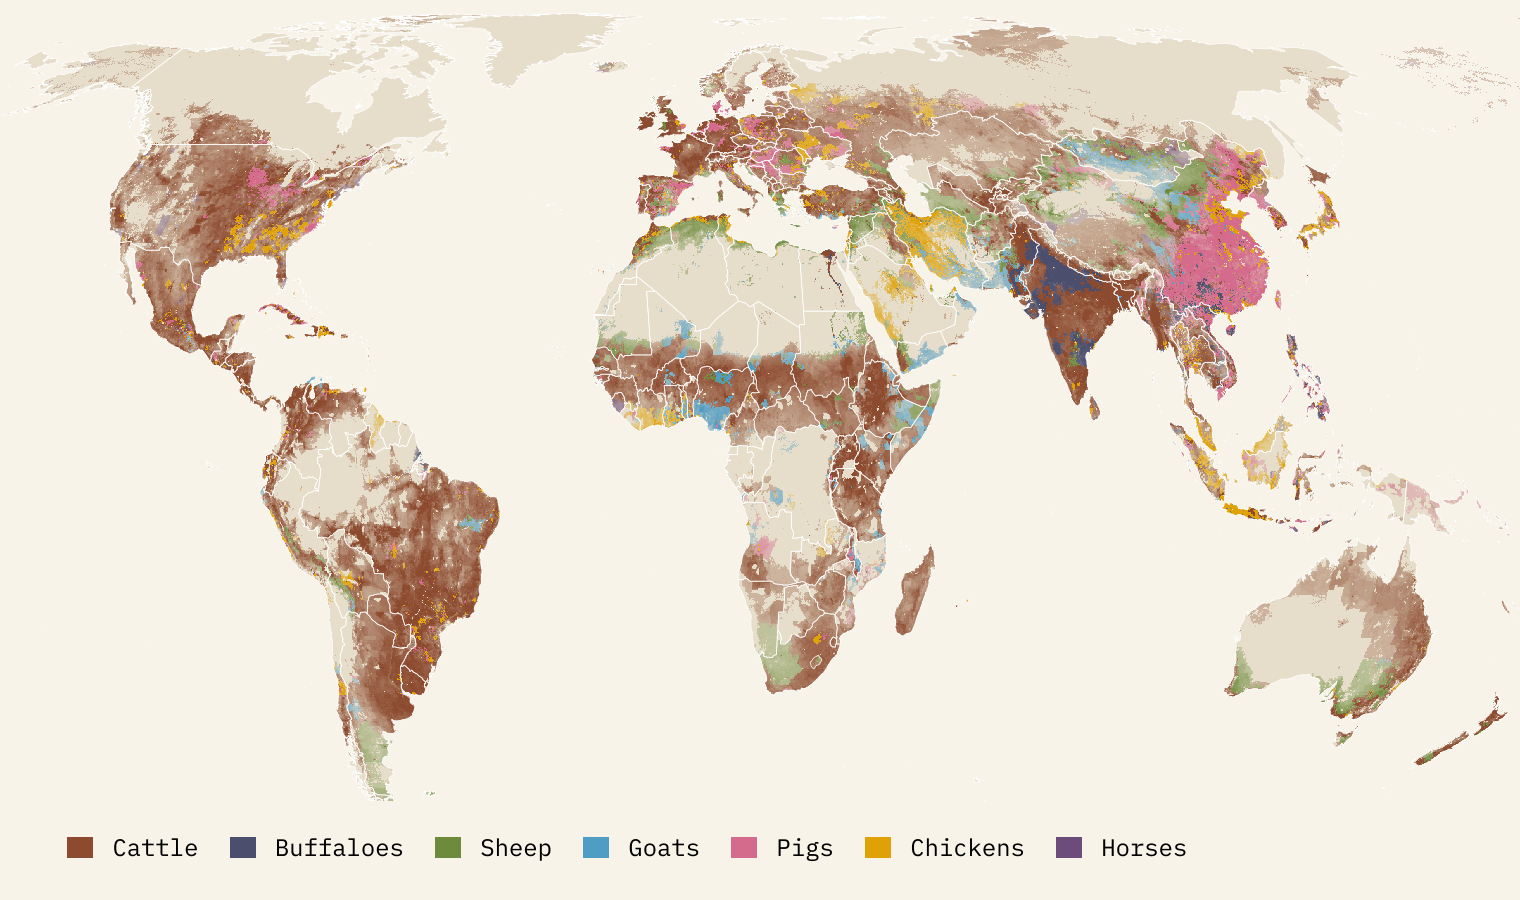
\includegraphics[width=\textwidth]{f_main_map.png}
\caption{Main farm animal by livestock units in each 10 km cell, 2015 (GLW 4 with FAOSTAT livestock unit factors). Paler cells have fewer livestock units per km\textsuperscript{2}; cells with less than one are blank.}\label{fig:main}\end{figure}

\subsection{Britain and Ireland}
The United Kingdom has 31.0 million sheep (2024), more than any other European country by FAOSTAT's count other than Turkey, which spans Europe and Asia, as well as 9.4 million cattle, 4.7 million pigs and 167 million chickens. By livestock units its main animal is cattle (57\%), then sheep (21\%). The grid divides the country by its uplands (Figure~\ref{fig:uk}, Table~\ref{tab:uk}): Wales has 9\% of the UK's land and 26\% of its sheep, 420 per km\textsuperscript{2}, 3.5 times England's density, and Powys alone has 10\% of UK sheep (663 per km\textsuperscript{2}). Cattle are densest in Northern Ireland (109 per km\textsuperscript{2}) and in Cheshire, Cornwall and Somerset. England has 81\% of UK pigs, the largest numbers in North Yorkshire and Norfolk and the highest density in the East Riding of Yorkshire (136 per km\textsuperscript{2}); Herefordshire (4,039 per km\textsuperscript{2}) and Lincolnshire have the most chickens per km\textsuperscript{2}. Cattle are the main animal in 74 of 88 counties, sheep in 9, pigs in 3 and chickens in 2. Ireland has 1.2 cattle per person, and cattle make up 88\% of its livestock units.

\begin{figure}[tbp]\centering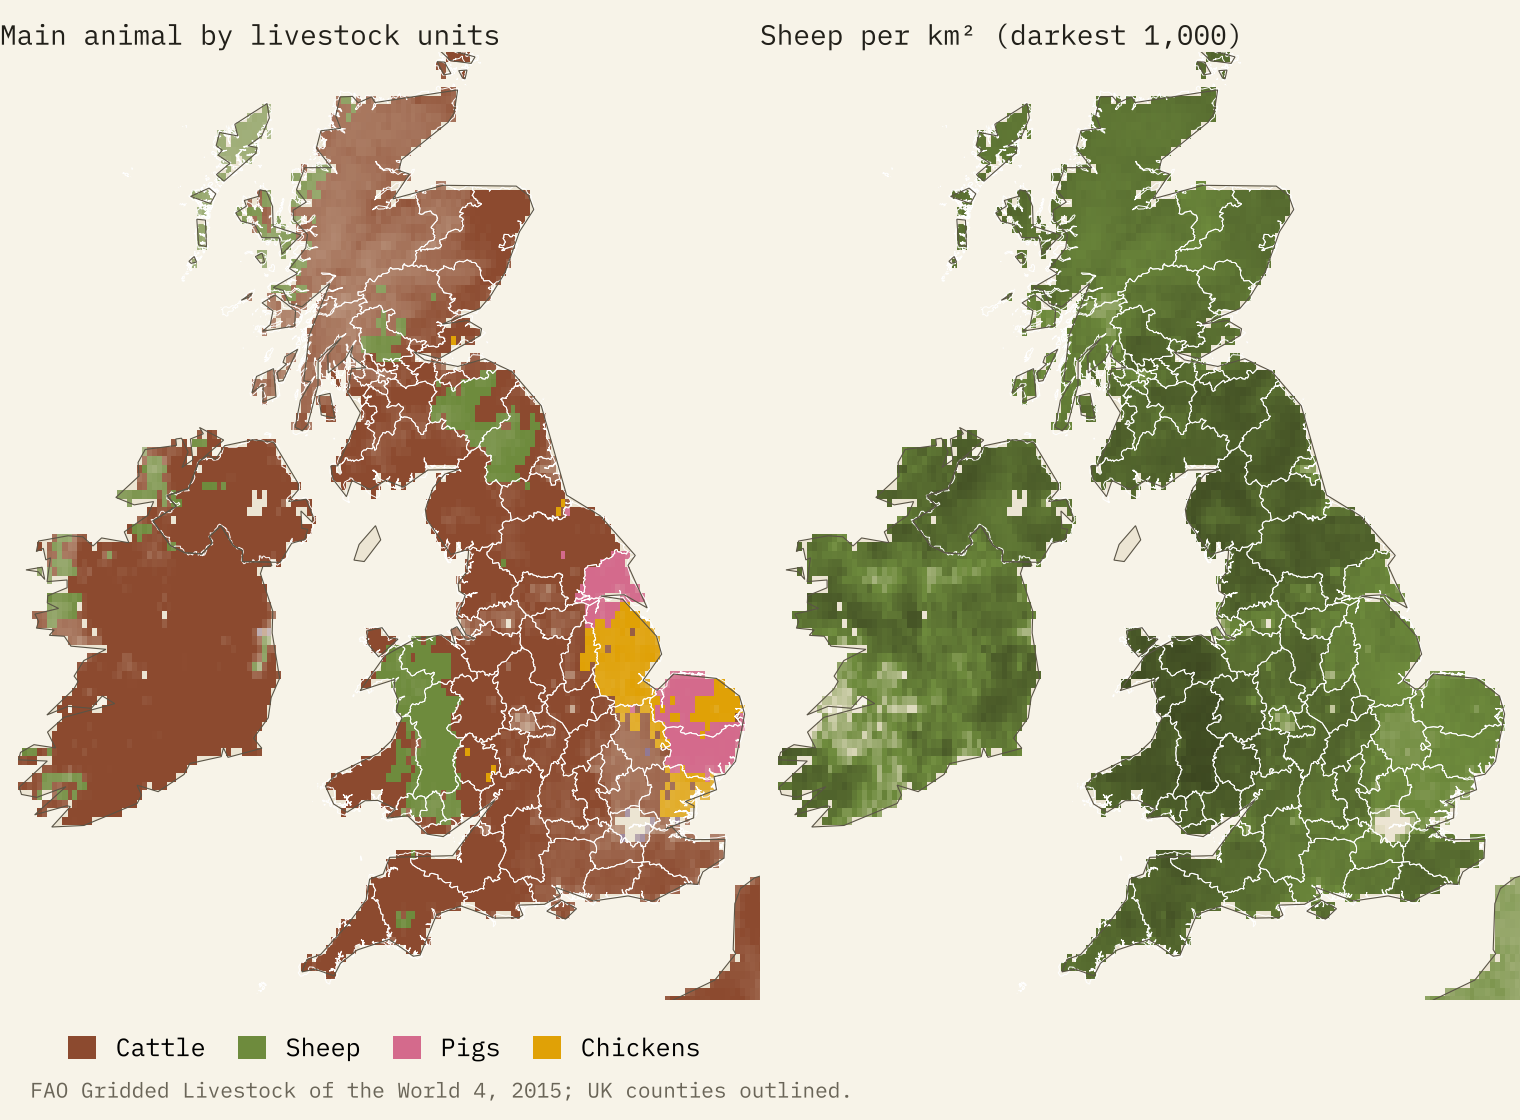
\includegraphics[width=\textwidth]{f_britain_ireland.png}
\caption{Britain and Ireland: main animal by livestock units and sheep density, 2015 (GLW 4), with UK counties.}\label{fig:uk}\end{figure}

\begin{table}[tbp]\centering\small\caption{UK nations in the grid, 2015 (GLW 4; millions of head, and head per km\textsuperscript{2}).}\label{tab:uk}\setlength{\tabcolsep}{4pt}\begin{tabular}{lrrrrrrr}\toprule Nation & km\textsuperscript{2} & Sheep & Cattle & Pigs & Chickens & Sheep/km\textsuperscript{2} & Cattle/km\textsuperscript{2}\\\midrule
England & 129,620 & 15.6 & 5.50 & 3.84 & 120.3 & 120 & 42\\
Scotland & 78,061 & 7.1 & 1.78 & 0.44 & 11.5 & 91 & 23\\
Wales & 20,653 & 8.7 & 1.06 & 0.03 & 7.0 & 420 & 51\\
Northern Ireland & 14,202 & 1.9 & 1.55 & 0.43 & 17.7 & 137 & 109\\
\midrule United Kingdom & 242,537 & 33.3 & 9.89 & 4.73 & 156.5 & 137 & 41\\
\bottomrule\end{tabular}\end{table}

\section{Discussion}
The map confirms some familiar pictures and corrects others. The most numerous large farm animal is not the sheep of popular imagination but the cow, and the most numerous of all is the chicken, with 3.4 alive for every person. The growth since 1961 has been in animals that turn feed into meat quickly (chickens, ducks, pigs) and in the hardy small ruminants of dry countries (goats, and camels), while working animals have declined. The geography follows: housed animals crowd onto a few per cent of the land near feed, people and processing, while cattle, sheep and goats spread across grasslands, drylands and hills. Countries where animals outnumber people are almost all dry or grassy and thinly peopled, from Mongolia and the Sahel to Uruguay, Australia and New Zealand.

New Zealand shows that even the most familiar picture can be out of date: it has three times fewer sheep than in 1982. The United Kingdom remains one of the great sheep countries of Europe, but its sheep are concentrated in the hills of Wales, northern England and southern Scotland, while its pigs and poultry are on the arable plains of the east.

\section{Limitations}
First, the grid is a model. GLW shares census totals among cells using predicted densities, so within each census area the pattern reflects the covariates rather than observed farms; where census areas are large, as in parts of Africa and Asia, cells can look smooth or blocky, and animals may be spread thinly over remote land. Second, the grid is for 2015 only, while country counts run to 2024; the two are not combined over time. Third, FAOSTAT stocks are official national figures and FAO estimates of uneven quality; nomadic and smallholder herds are hard to count, and some series are imputed. Fourth, stocks are animals alive at one time: broiler chickens live a few weeks, so the number raised in a year is far higher than the number alive. Fifth, livestock units are a rough common currency and the `main animal' depends on the factors chosen; by head, chickens would lead almost everywhere. Sixth, the UK county figures depend on the grid's own census inputs and on sharing 10 km cells by area. Finally, wild animals, reindeer, farmed fish and insects are not included.

\section{Conclusion}
Open data from FAO make it possible to map the world's farm animals in detail and to tell a clear story of change: many more chickens, goats and pigs, relatively fewer cattle per person, and fewer working animals. The atlas lets readers explore that story for any place on Earth, with the caveats of a modelled grid kept in view.

\section*{Data and code availability}
The interactive atlas is at \url{https://maps.tristanhotham.com/livestock-map/}. Data and code are at \url{https://github.com/Tristan-Hotham/livestock-map} and archived with this paper at \url{https://doi.org/10.5281/zenodo.23842985}. Derived data and text are released under CC BY 4.0 and code under the MIT licence. GLW 4 and FAOSTAT are CC BY 4.0 (FAO); World Bank data are CC BY 4.0; Natural Earth is in the public domain.

\section*{AI statement}
I wrote the text, with drafting and editing assistance from Claude (Anthropic), which also helped prepare the analysis code. I reviewed and checked all text and results.

\begin{thebibliography}{9}
\bibitem[FAO(2026)]{faostat} FAO (2026) FAOSTAT: Crops and livestock products (QCL), Livestock patterns (EK) and Land use (RL). Food and Agriculture Organization of the United Nations, Rome. CC BY 4.0. \url{https://www.fao.org/faostat/}
\bibitem[Gilbert et al.(2018)]{gilbert2018} Gilbert, M., Nicolas, G., Cinardi, G., Wint, G. R. W., Vanwambeke, S. O. and Robinson, T. P. (2018) Global distribution data for cattle, buffaloes, horses, sheep, goats, pigs, chickens and ducks in 2010. \emph{Scientific Data}, 5, 180227. \url{https://doi.org/10.1038/sdata.2018.227}
\bibitem[Gilbert et al.(2022)]{glw4} Gilbert, M. et al. (2022) Gridded Livestock of the World (GLW 4): global distribution of cattle (doi:10.7910/DVN/LHBICE), sheep (VZOYHM), goats (YYG6ET), pigs (CIVCPB), chickens (SXHLF3), buffaloes (I1WCAB), horses (JJGCTX) and ducks (S9ONXV) in 2015. Harvard Dataverse, CC BY 4.0. \url{https://doi.org/10.7910/DVN/LHBICE}
\bibitem[Natural Earth(2026)]{naturalearth} Natural Earth (2026) Admin 0 countries (1:50m) and populated places. Public domain. \url{https://www.naturalearthdata.com/}
\bibitem[Nicolas et al.(2016)]{nicolas2016} Nicolas, G., Robinson, T. P., Wint, G. R. W., Conchedda, G., Cinardi, G. and Gilbert, M. (2016) Using random forest to improve the downscaling of global livestock census data. \emph{PLoS ONE}, 11(3), e0150424.
\bibitem[Robinson et al.(2014)]{robinson2014} Robinson, T. P., Wint, G. R. W., Conchedda, G., Van Boeckel, T. P., Ercoli, V., Palamara, E., Cinardi, G., D'Aietti, L. and Gilbert, M. (2014) Mapping the global distribution of livestock. \emph{PLoS ONE}, 9(5), e96084.
\bibitem[World Bank(2026)]{wbpop} World Bank (2026) World Development Indicators: population, total (SP.POP.TOTL), as packaged at \url{https://github.com/datasets/population}. CC BY 4.0.
\end{thebibliography}
\end{document}
